\section{Experiment}

F�r die Simulation wurden die sich im Anhang A befindlichen Eingabedaten benutzt. Nun folgt eine kurze Erkl�rung der Gr��e. Die Daten entstammen aus \cite{tautz2007phaenomen, genersch2010honey, tautz2013bee}. Falls bestimmte Werte nicht bekannt oder in diesem Falle nicht nutzbar waren, wird der Grund der �nderung nachfolgend angegeben.

Ein Bienenstock beherbergt normalerweise ungef�hr 50000 Bienen. Aus Performancegr�nden musste diese Anzahl reduziert werden, da eine Simulation auf der verf�gbaren Hardware ansonsten nicht m�glich gewesen w�re. Die Eierlegerate der K�nigin ergibt sich aus der durchschnittlichen Rate von 2000 Eiern pro Tag. Das entspricht etwa einer Rate von einem Ei alle 43s. Die initiale Erkrankungsrate wurde so gew�hlt, dass ungef�hr eine Biene pro Stock zum Simulationsbeginn erkrankt ist (bei 1000 Bienen pro Stock). Neben den Nektar sammelnden Arbeiterinnen gibt es noch Drohnen und Arbeiterinnen, die sich um die Brutpflege k�mmern. Der Anteil der Bienen, die Nektar sammeln, betr�gt in etwa 55\%. Sobald 75\% der Bienen eines Stocks ausgestorben sind, zerf�llt der ganze Stock. 

Die Ansteckungswahrscheinlichkeit wurde so gew�hlt, dass die Populationen eine bestimmte Zeit �berleben, aber bis zum Ende des Simulationszeitraums (1 Jahr) gerade alle abgestorben sind. Bei Werten kleiner als 0.0005 kam es zum �berleben einiger St�cke zum Simulationsende. Werte gr��er als 0.0005 f�hrten dazu, dass die Bienenst�mme wesentlich fr�her als 1 Jahr verstarben. Die Bienen bewegen sich im Flug mit 5 km/h fort. Eine Biene lebt im Mittel 45 Tage. Die tats�chliche Lebenszeit liegt zwischen 40 und 50 Tagen. Die Zeit bis zum Ausbruch der Krankheit betr�gt 2 Tage. Nach dem Ausbruch �berlebt eine Biene noch 2 Tage. Die Zeit, die eine Sammlerin zum Nektarsammeln ben�tigt, betr�gt eine halbe Minute. Nachdem eine Biene zu ihrem Stock zur�ckkehrte, gibt sie den Nektar ab und ruht sich danach aus. Daher dauert die Nektarabgabe so lange. Eine Biene kann pro Flug 40 Einheiten Nektar transportieren. Falls der Nektar einer einzelnen Blume aufgebraucht ist, fliegt eine Biene zur n�chsten Blume. Es besteht eine Wahrscheinlichkeit, dass Bienen nach dem Nektarsammeln zum falschen Stock fliegen. Es wird zuf�llig ein Stock aus einem bestimmten Radius ausgew�hlt. St�cke in der N�he des Heimatstocks haben eine h�here Wahrscheinlichkeit ausgew�hlt zu werden. Der Heimatstock erh�lt die h�chste Wahrscheinlichkeit.

Die Anzahl der Blumen pro Biene wurde so ermittelt, dass die Blumen zu jeder Zeit �ber Nektar verf�gen und es zu keinen Engp�ssen kommt. Nach Beginn der Simulation pegelt sich der verf�gbare Nektar bei 50\% ein.
\begin{figure}[t]
	\begin{center}
    	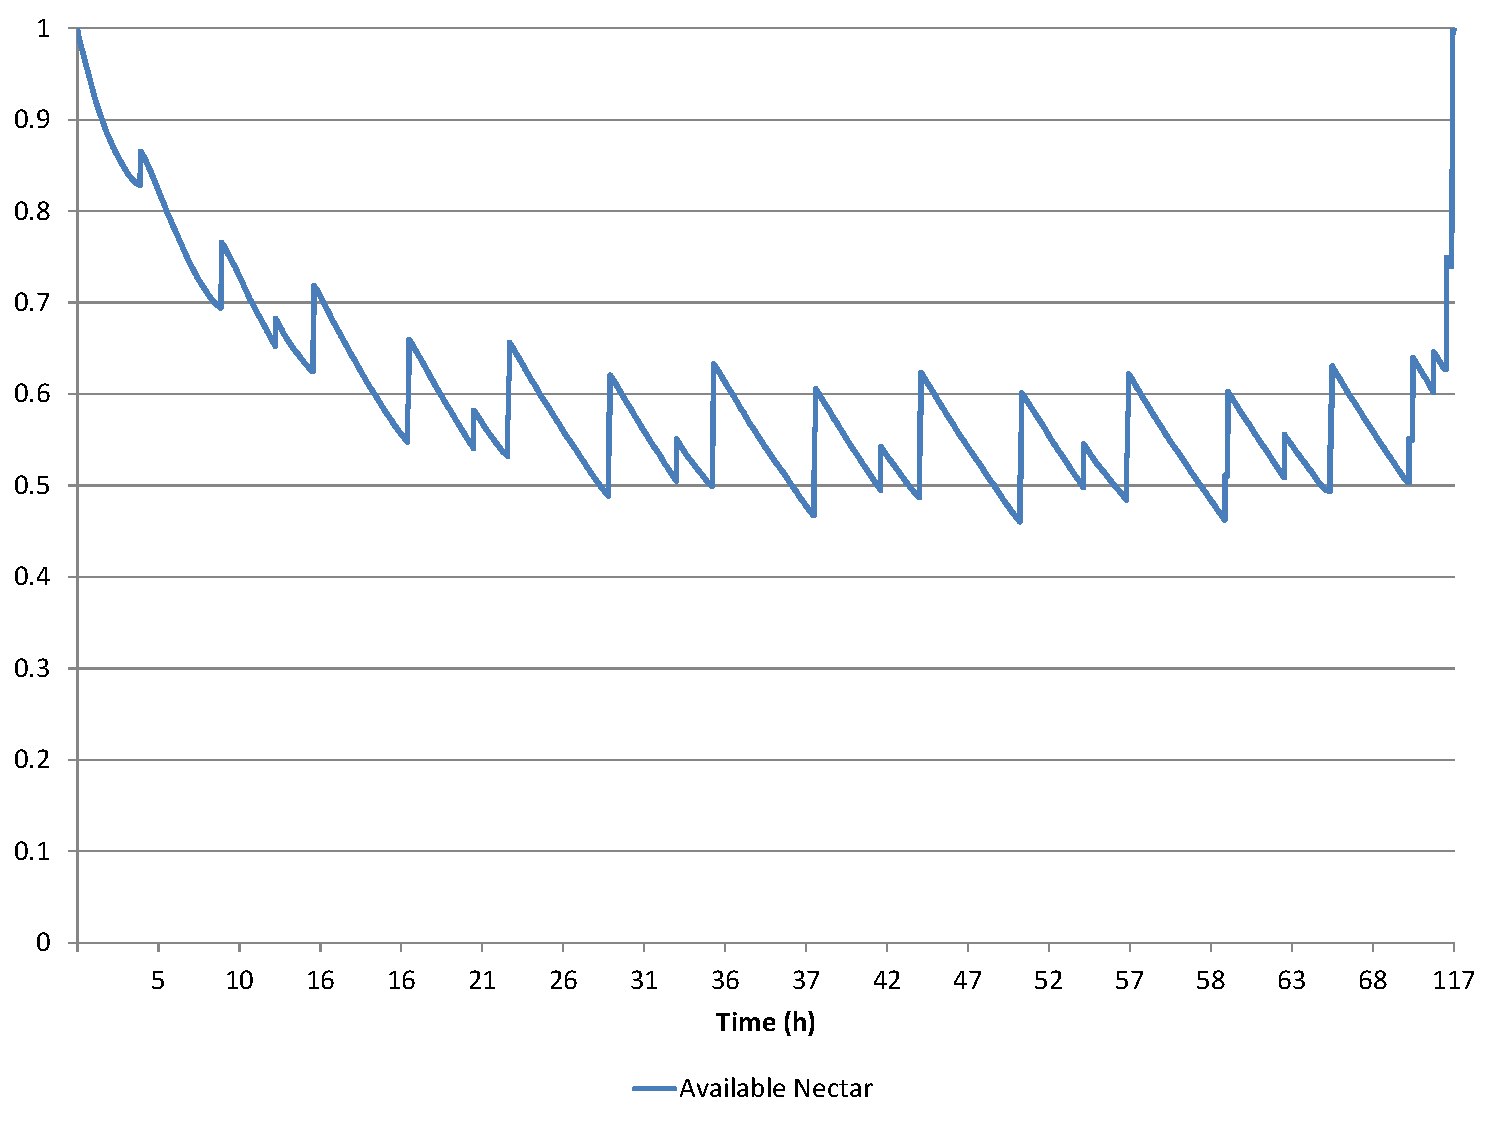
\includegraphics[width=1\linewidth]{available_nectar}
  \caption{�ber Simulationszeit verf�gbare Nektarmenge.}
  \label{img:available_nectar} 
	\end{center}
\end{figure}
\textbf{Missing: Nektarmenge, woher?}. Eine Blume ben�tigt einen Tag um den Nektar vollst�ndig zu regenerieren.
